\clearpage
\chapter{}
\section{Phylogenetic Analyses}
%%%%%%%%%%%%%%%%%%%%%%%%%%%%%%%%%%%%%%%%%%%%%%%%%%%%%%%%%%%%%%%%%%%%
\addcontentsline{toc}{subsection}{Summary}
\subsection*{SUMMARY}
\hrule
Here is a summary of some results from phylogenetic analyses, and some pretty figures.

%% FIGURE %%
\begin{figure}[ht]
\centering
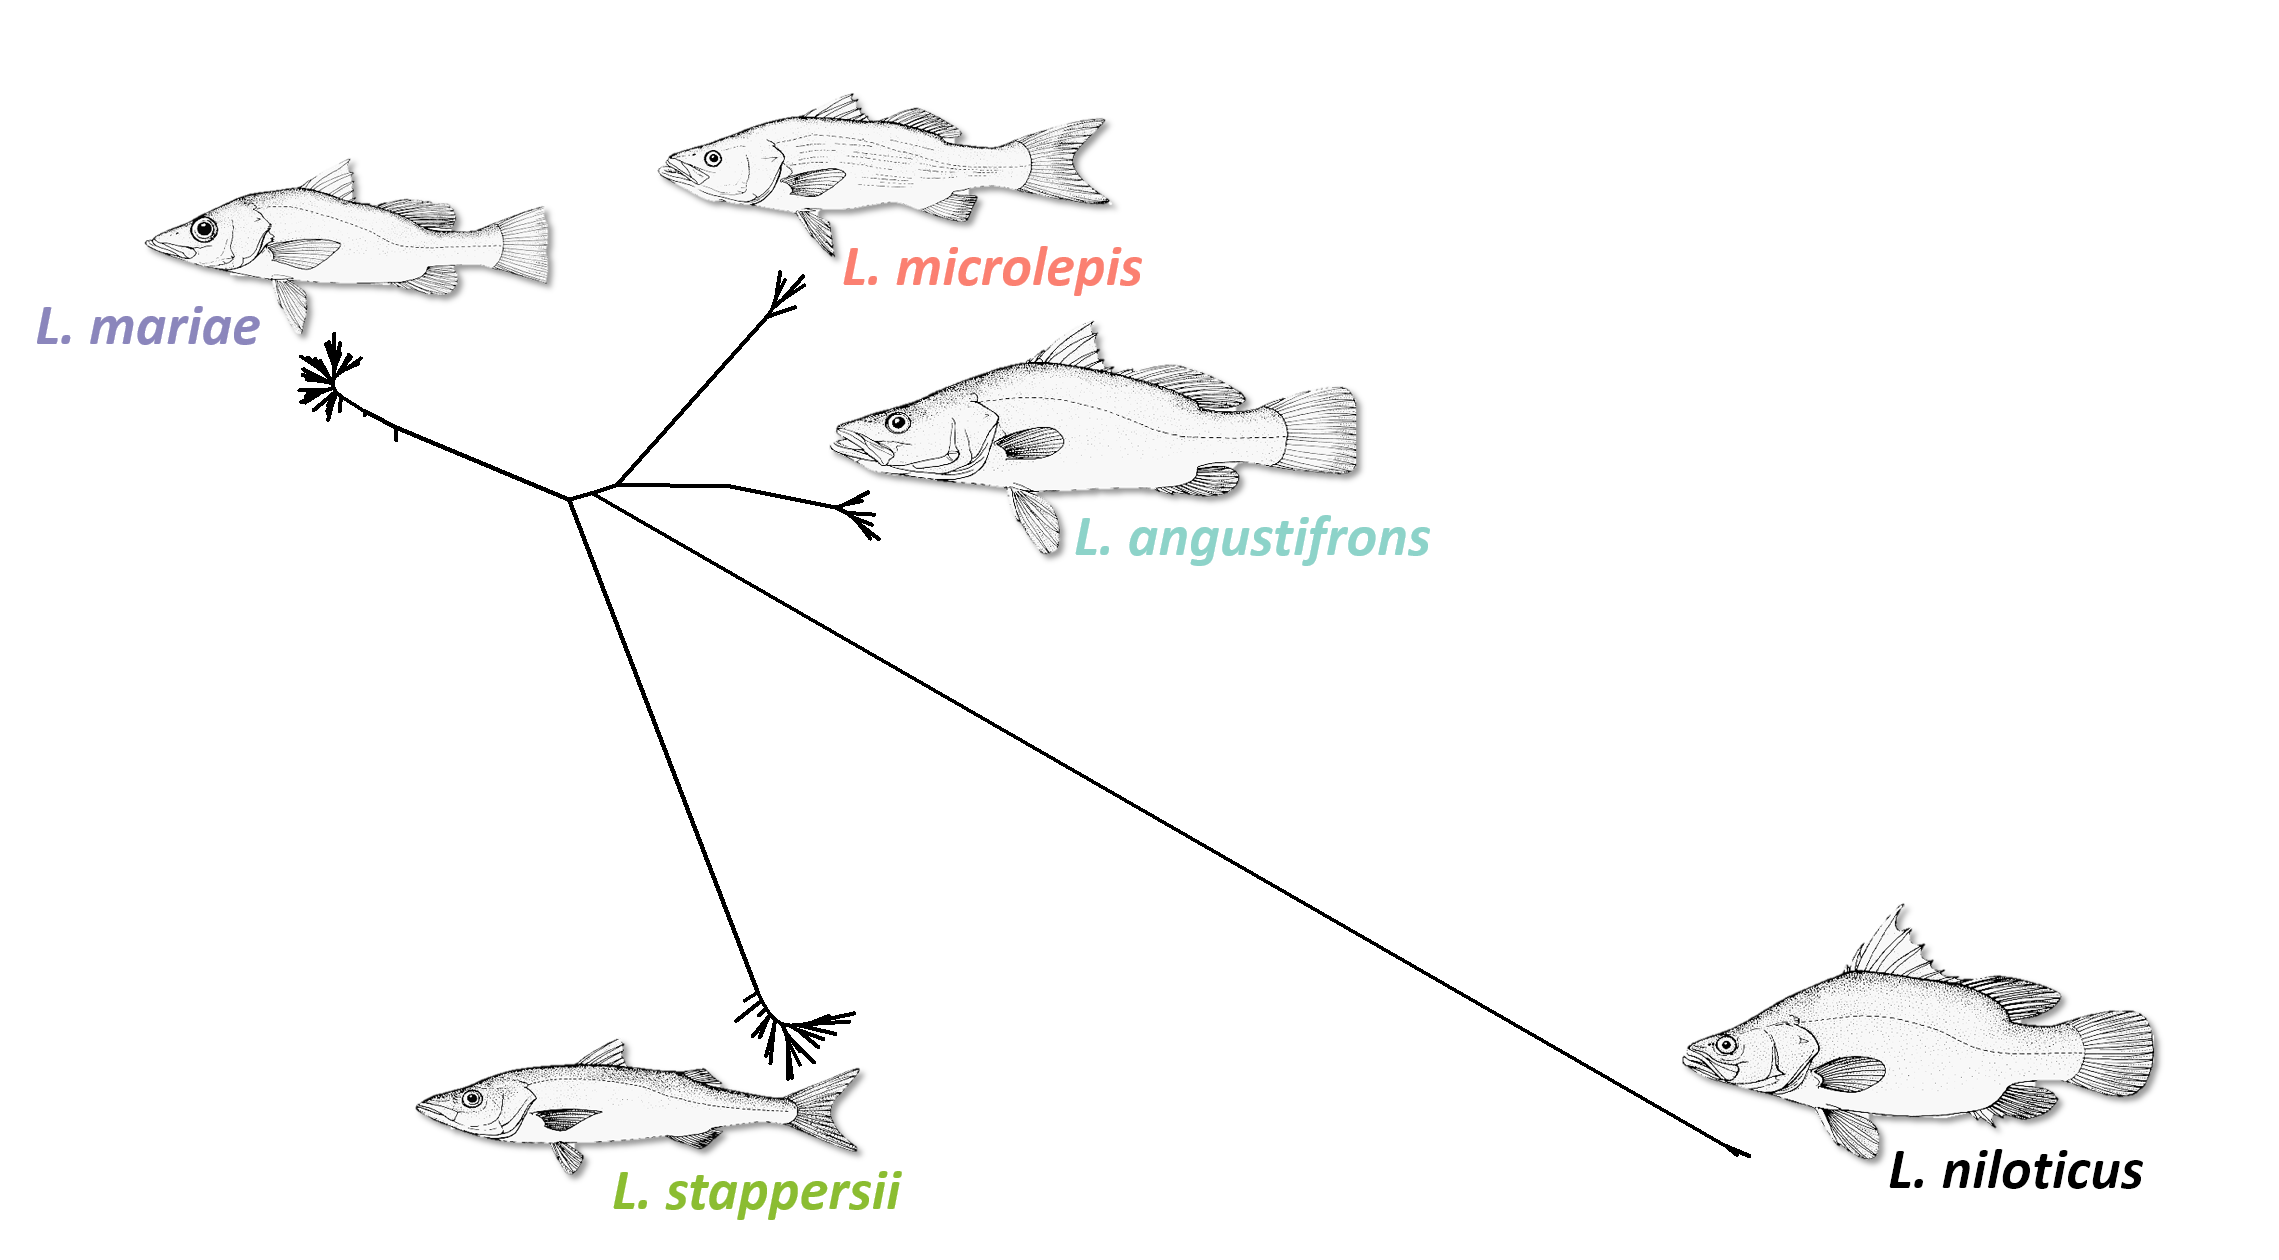
\includegraphics[width=0.7\textwidth]
{figures/lates_phylogeny_020218.png}\caption{\label{fig:raxml-phylogeny} Preliminary RAxML phylogeny based off of \textit{Lates} GBS data, aligned to the \textit{L. calcarifer} genome, and following filtering for $\leq$ 20\% missing data and MAF $\leq$ 0.01. These SNPs were not filtered for linkage disequilibrium.}
\end{figure}
%%%%

%%%%%%%%%%%%%%%%%%%%%%%%%%%%%%%%%%%%%%%%%%%%%%%%%%%%%%%%%%%%%%%%%%%%%
\subsection*{NEXT TO-DO}
\hrule

\begin{enumerate}
\item Item 1
\end{enumerate}

%%%%%%%%%%%%%%%%%%%%%%%%%%%%%%%%%%%%%%%%%%%%%%%%%%%%%%%%%%%%%%%%%%%%
\addcontentsline{toc}{subsection}{Log}
\subsection*{LOG}
\hrule
%%%%%%%%%%%%%%%%%%
\hrulefill
\begin{large}\textbf{5 March 2018}\end{large} \\
%%%%%%%%%%%%%%%%%%
Here's an entry with a two-part figure.

%% FIGURE %%
\begin{figure}[htb]
\centering
\begin{subfigure}{.45\textwidth}
  \centering
  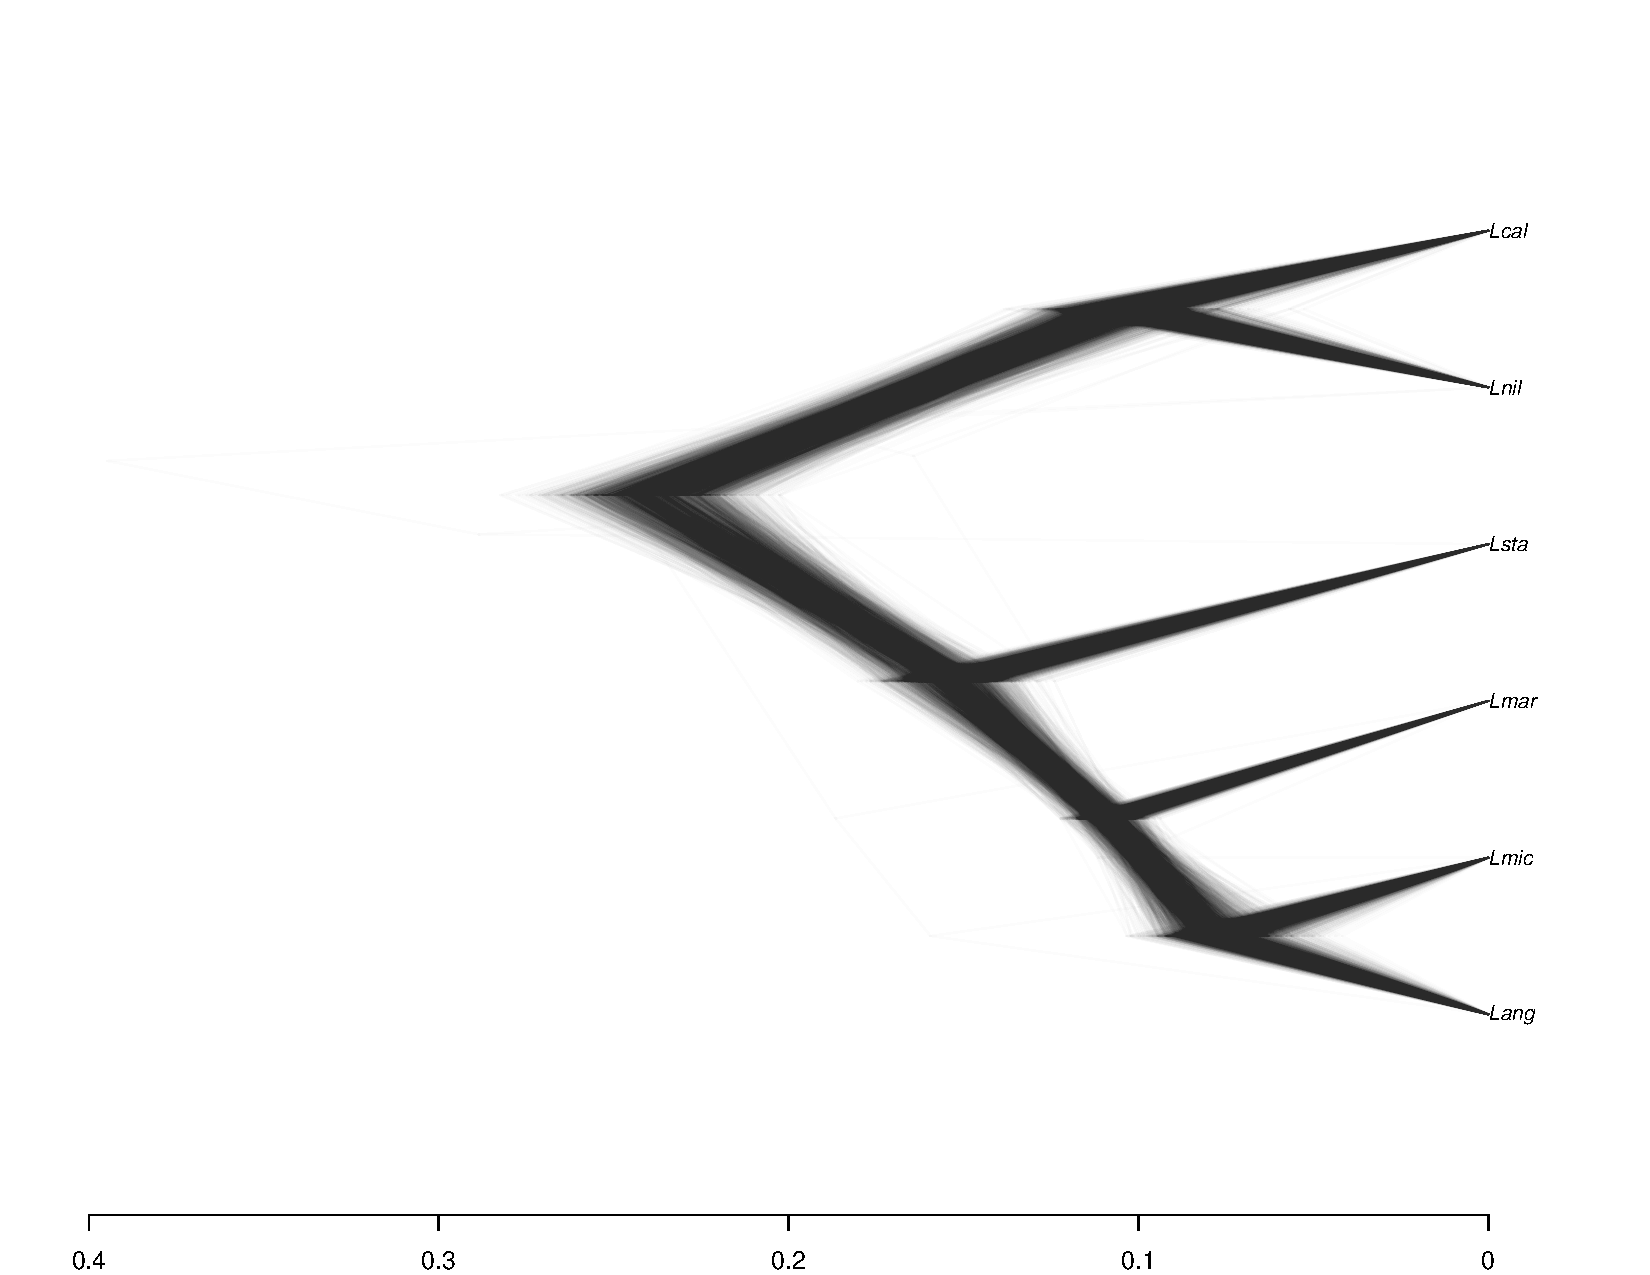
\includegraphics[width=.95\linewidth]{figures/densitrees_030318.pdf}
  \caption{Densitrees from posterior}
  \label{fig:030318-densitree}
\end{subfigure}%
\begin{subfigure}{.55\textwidth}
  \centering
  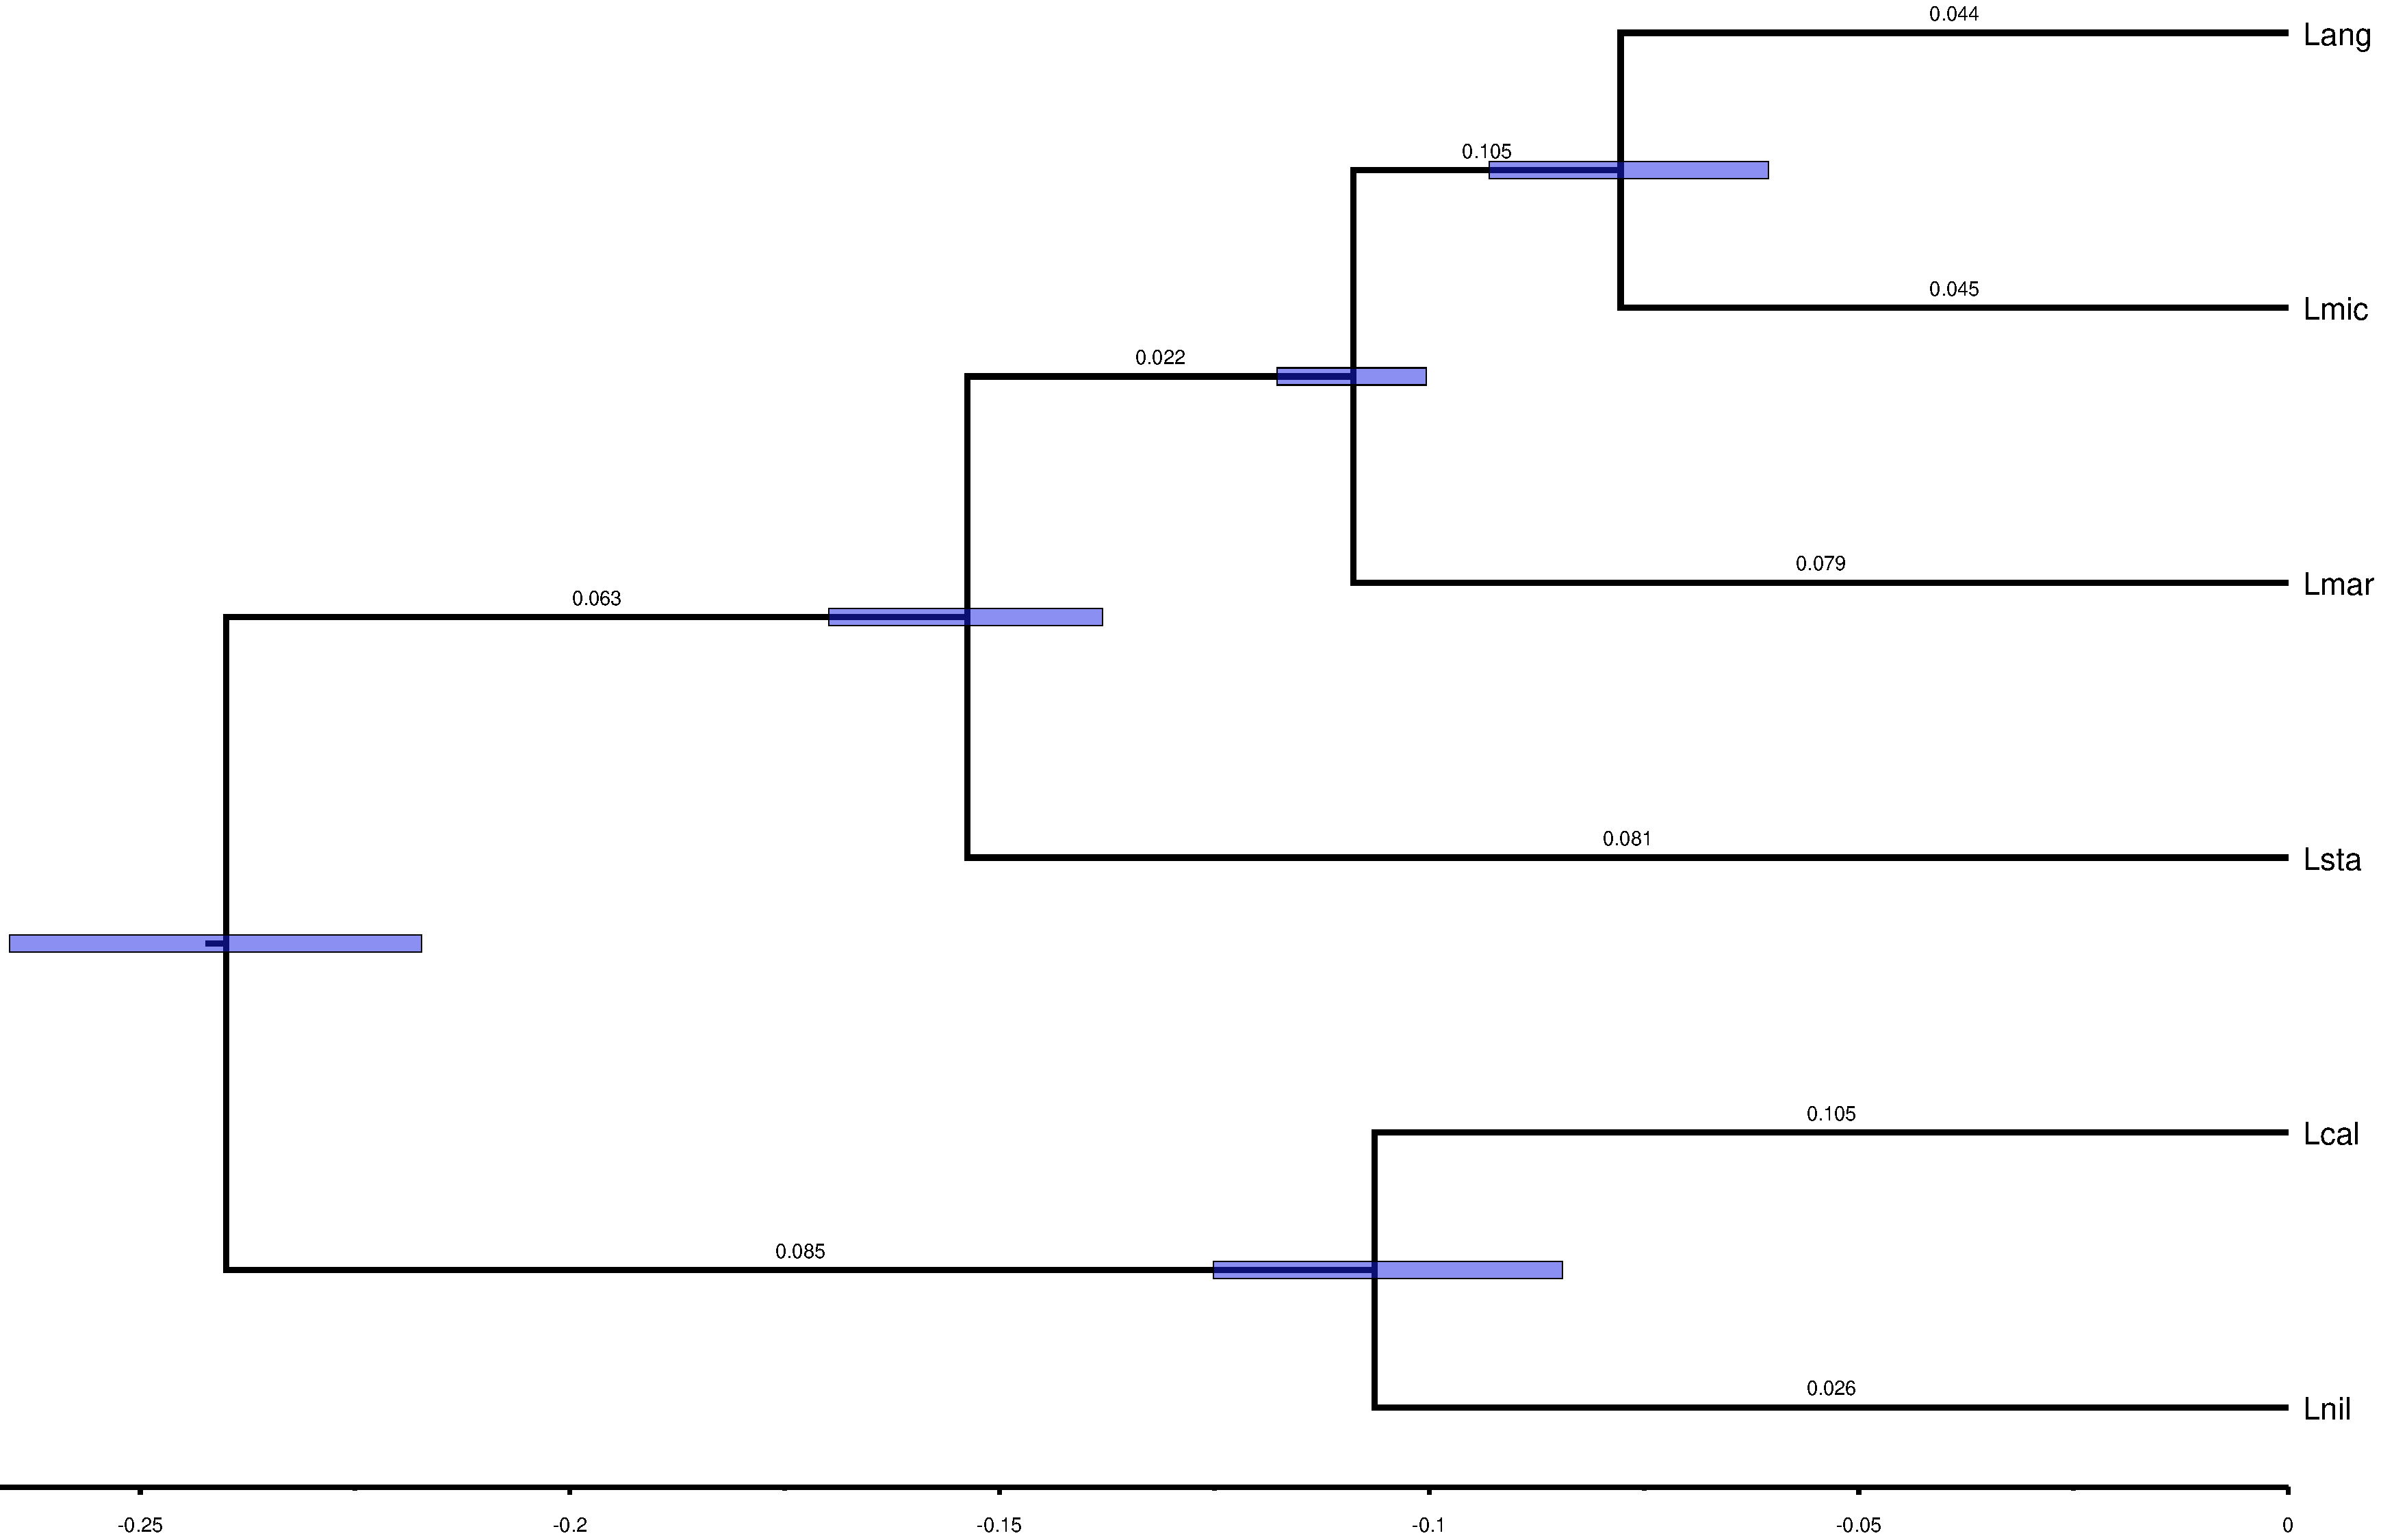
\includegraphics[width=.95\linewidth]{figures/snapp_calcar_thin50k_small_030318_tree.pdf}
  \caption{Consensus tree}
  \label{fig:030318-tree}
\end{subfigure}
\caption{Trees from \texttt{SNAPP} runs, followed by summary in \texttt{TreeAnnotator}, run for 3 million MCMC iterations using parameter file \texttt{snapp\_calcar\_thin50k\_small\_030318.xml}. Data are SNPs called from GBS reads aligned to the \textit{L. calcarifer} genome (v3, chromosome-level), thinned to a minimum distance of 50,000bp between SNPs and with invariant sites removed (4,696 SNPs total). Values on branches show the median theta value, and purple bars show 95\% HPD for node depths.}
\label{fig:tree-annotator-calcar}
\end{figure}
%%%%%

%%%%%%%%%%%%%%%%%%%%%%%%%%%%%%%%%%%%%%%%%%%%%%%%%%%%%%%%%%%%%%%%%%%%%
\bibliographystyle{agsm}
\bibliography{Mendeley}